\chapter{State of the Art in Factoid Question Answering}
\label{ch:survey}

The research in Question Answering has been proceeding in several,
largely independent, directions.  The main division is between QA
on structured knowledge bases (typically graph databases like the
semantic web) and QA on unstructured text corpora (typically
Wikipedia, ClueWeb, large amounts of news articles, or even
a web search).

Below, we survey the recent activity in these fields.
For a historical viewpoint, we refer the reader to
\cite{SurveyWang}, \cite{SurveyAllam} and \cite{SurveyLopeza}.


\section{Structured Data QA}
\label{sec:structured}

When answering questions on structured data, we can further
consider either helping users access relational databases (Natural Language Interface to Databases; NLIDB)
or finding matching relationships in the linked data graph of semantic web (Ontology-based Question Answering; QALD).

We are not aware of any significant recent work in the NLIDB domain
that would be based on well defined, published dataset and rigorously
evaluate results --- most research concerns building auxiliary systems
that augment human database experts. \citep{BergamaschiKeymantic, BlunschiSODA}
We do not consider this branch of research further.

QALD is much richer field of research, with yearly challenges \citep{QALD} and
popular reference datasets Free917 \citep{Free917} and WebQuestions \citep{WebQuestions}.%
\footnote{In the past, closed-domain datasets like GeoQuery were also popular.}
The reference knowledge base is typically Freebesa \citep{Freebase},
which holds a large amount of open domain real-world facts.%
\footnote{Freebase has been phased out into legacy state at this point.
	WikiData is set to replace it, but the migration of knowledge
	is still ongoing.}
QALD is one of the benchmarks for the semantic parsing task \citep{SPIntro}, aiming
to map a naturally phrased question to a logical form (to be in this case
executed as a graph query on a knowledge base).
\citep{SPBerant2014Paraphrase, Semantic2014Bordes}

\citep{Semantic2014Bordes} proposed a classification of QALD methods
that we adopt, outlining two general paradigms:

\begin{quote}
\textbf{Information
Retrieval (IR)} systems first retrieve a broad set of candidate answers by querying
the search API of KBs with a transformation of the question into a valid
query and then use fine-grained detection heuristics to identify the exact answer
(Kolomiyets survey 2011, Unger et al. 2012 templates, \citep{TreeFreebase2014Yao} TODO).
On the other hand, \textbf{Semantic Parsing (SP)} methods focus on the correct
interpretation of the meaning of a question by a semantic parsing system. A
correct interpretation converts a question into the exact database query that
returns the correct answer. \citep{Semantic2013Berant, SPBerant2014Paraphrase, OQA}
\end{quote}

These two strategies have been also compared in detail in \cite{FreebaseQA2014Yao}
and appear roughly comparable in accuracy.

\subsection{Dataset and Evaluation}

The most popular question dataset is WebQuestions \citep{WebQuestions},
which contains 3778 training and 2032 testing questions generated
automatically by a combination of Google Suggest API and Freebase%
\footnote{Note that no fixed version of Freebase is used.
	Since the answers are typically not a subject of temporal drift,
	it is unlikely that different Freebase snapshots would yield
	significant differences, but we are not aware of any study confirming this.}
and with the gold standard answers manually produced by Amazon Mechanical Turk workers.%
\footnote{The gold standard has noise level of about $5\%$ questions,
	based on manual error analysis of a Google QA test on a movies sub-sample.}
Answers are always Freebase entities --- never relations themselves,
literals like numerical quantities, metadata like counts, or whole sentences.
Sometimes, the correct answers are lists of entities.
Extra measurements on customized versions of TREC (see below) and WikiQuestions
datasets are also sometimes published.

There is no complete consensus on benchmarking metrics in this task,
owing to different strategies in the systems.
In the simplest case, a single query is generated for every question
and its result is matched with the gold standard
\citep{Semantic2013Berant}, then we may measure just the \textit{accuracy}
(i.e.\ proportion of correctly answered questions).

However, most systems generate a ranked list of candidate answers.
IR list measures are sometimes used \citep{Fader2013Paraphrase,Semantic2014Bordes}:
\textit{MRR} (Mean Reciprocial Rank) can capture the average rank the correct answer appears at,
while \textit{MAP} (Mean Average Precision) is not as intuitively interpretable, but generalizes
even to a scenario with multiple expected correct answers.
Aside of that, an option is to consider only correctness of the best answer,
introducing measures
\textit{precision@1} as the proportion of questions that have a correct answer ranked first
(and, if some questions generate no answers, \textit{recall@1} and \textit{F$_1$@1}).

However, the official WebQuestions evaluation script
of \citep{Semantic2013Berant} considers the complete set
of returned answers --- this fits e.g. \citep{TreeFreebase2014Yao},
where answer correctness is treated as a binary classification problem
and answers classified as true are returned (e.g.\ with logistic regression
output larger than 0.5 as proposed in \cite{FreebaseQA2014Yao}).
We term these \textit{answer precision} and \textit{answer recall}.
The most common measure shared by most papers is F$_1$
(with recall as a proportion of correct answers found).
However, even this measure comes in two variations:
\textit{F$_1$ (Berant)} is average of precision/recall harmonic means per question,%
\footnote{This is about the same as the accuracy in \cite{Semantic2013Berant} style systems.
When comparing using this measure in ranked-answers systems,
a single answer is often forced even if none would be produced for the question otherwise. \citep{FreebaseQA2014Yao}}
while \textit{F$_1$ (Yao)} is harmonic mean of answer precision and recall computed across all questions,
which gives an incentive to a system not to answer some questions.

Ultimately, the difference between the two approaches is how strictly are answers
to list-based questions evaluated and what policy does a system choose for
picking answers to be evaluated (first, all with score above 0.5, etc.).
We recommend that to facilitate comparison between systems that make different choices
and possibly do not emphasize list performance,%
\footnote{Below, we show that in unstructured QA, it is common to disregard list-based performance.
Therefore, this aspect is important to hybrid systems.}
future systems report both metrics that give credit to the best rank of at least
a single list element (F$_1$@1, MRR), and metrics that strictly rate the appearance
of all list elements and treat all generated answers as a proposed list (F$_1$ (Berant, Yao), MAP).
(Systems which generate an answer to each question will have F$_1$@1 equal
to precision@1 and recall@1.)

\begin{figure}[t]
%% increase table row spacing, adjust to taste
%\renewcommand{\arraystretch}{1.3}
\centering
\begin{tabular}{|c|ccc|cccc|}
\hline
System & F$_1$@1 & F1 (Berant) & F1 (Yao) \\ \hline
\cite{OQA} &
---              & ---         & (35.0\%) \\
\cite{TreeFreebase2014Yao} &
35.4\%           & 33.0\%      & 42.0\%   \\
\cite{Semantic2014Bordes} &
40.4\%           & 39.2\%      & 43.2\%   \\
\cite{LeanFreebaseYao} &
---              & 44.3\%      & 53.5\%   \\
\cite{Aqqu} &
---              & 49.4\%      & ---      \\
\hline
\cite{Semantic2013Berant} &
35.7\%           & 35.7\%      & ---      \\
\cite{MTBao2014} &
37.5\%           & 37.5\%      & ---      \\
\cite{SPBerant2014Paraphrase} &
39.9\%           & 39.9\%      & 43.0\%   \\
\cite{STAGG} &
---              & 52.5\%      & ---      \\
\hline
\end{tabular}
\vspace*{-0.2cm}
\caption{Benchmark results of structured KB systems on the WebQuestions dataset using Freebase.
Values in parenthesis have caveats like subsampling or manual evaluating.}
\label{fig:structcompare}
\end{figure}

\subsection{Information Retrieval Approach}

\textbf{Open Question Answering Over Curated and Extracted Knowledge Bases (OQA)} \citep{OQA}
	is a complex multi-stage system:
	the question is paraphrased (using mined operators),
	parsed to a KB query (by manual templates),
	the query rewritten (using mined operators again),
	and executed (on an ensemble of KBs including Freebase).
	On WebQuestions, F$_1$ (Yao --- probably) is reported at 35\%.
	Results on TREC were also reported, with F$_1$ 29\%.
	However, the answers were evaluated manually.
	The implementation is open source.

\textbf{Information Extraction over Structured Data: Question Answering with Freebase (Jacana Freebase)} \citep{TreeFreebase2014Yao}
	produces a set of fixed dependency-parse based question features.
	The question entity is linked to a Freebase concept using the Freebase Search API;
	Freebase concepts neighboring the question concept in the knowledge
	graph are identified;
	Freebase features are generated for all
	properties of each concept, the connecting relation and rank
	of the connecting relation predicted by a question-relation
	alignment model.  The alignment model is a bag-of-words
	naive bayes classifier that predicts the probability of a relation
	(or sub-relation) component based on the question tokens;
	it is trained on \textsc{ClueWeb} sentences that contain
	both the question and answer.
	Finally, composite features are built for all tuples of question and Freebase features
	and a logistic regression model predicts the most likely Freebase concept to answer.
	As \citep{FreebaseQA2014Yao} also further clarifies,
	on WebQuestion+Freebase, this scores F$_1$ (Yao) 42.0\%,
	with answer precision $38.8\%$ and answer recall $42.0\%$,
	and F$_1$@1 $35.4\%$.
	Without the alignment model, the system has F$_1$ (Yao) 36.9\%.
	The implementation is open source.

\textbf{Question Answering with Subgraph Embeddings} \citep{Semantic2014Bordes}
	considers the QA task as a problem of finding a vector embedding
	of the question and candidate answers such that the score --- a scalar product
	of these embeddings\footnote{That is, non-normalized cosine similarity of vectors.} ---
	is highest for the correct answer.
	Question embedding is produced by averaging word embeddings
	(as in Sec.~\ref{sec:embeddings}; word embeddings are trained from scratch),
	the embedding matrix was also trained to produce similar
	vectors for question paraphrases (based on WikiAnswers).
	Answers are embedded from high-dimensional binary encoding
	of entities and relations in the subgraph surrounding the answer
	and the path between the question and answer.
	To generate candidate answers, the immediate neighborhood of the question
	concept is explored, and in addition directional forrays are made based
	on score of embeddings of particular relations.
	Aside of WebQuestion training set, automatically produced 2 million
	questions from ClueWeb were included for training.
	WebQuestions+Freebase precision@1 is $40.4\%$ and
	full-result F$_1$ (Berant) is $39.2\%$ and F$_1$ (Yao) $43.2\%$.
	(In ensemble with \cite{SPBerant2014Paraphrase},
	$F_1$ is reported as $41.8\%$ (Berant) or $45.7\%$ (Yao).)

\textbf{Lean Question Answering over Freebase from Scratch (kitt.ai)} \citep{LeanFreebaseYao}
	is a simple approach that uses
	fuzzy matching of all question bigrams to link entities to Freebase concepts,
	sorts them in the Freebase Search API order,
	and predicts Freebase relations linking the concept with the answer
	by a bag-of-unigrams-and-bigrams logistic regression.
	On WebQuestions+Freebase, it scores F$_1$ (Berant) 44.3\%, F$_1$ (Yao) 53.5\%.
	On the training set, this approach had AP recall of $62\%$.

\textbf{More Accurate Question Answering on Freebase} \citep{Aqqu}
	is an end-to-end system that first aggressively
	links many potential question entities to Freebase concepts,
	then generates answer candidates by matching three pre-defined
	templates in the knowledge (including one that uses entity pairs).
	Answers are filtered based on trivial type checking,
	and scored based on Freebase relation(s) alignment with
	the question --- number of overlaping words, derived words,
	word vector embedding cosine similarities and indicator
	words in question trained by distant supervision
	(Wikipedia sentences that contain two entities connected
	with such relation in Freebase would often have the indicator
	word on the path between the entities in dependency parse).
	The answers are ranked using pairwise random forest ranker.
	On WebQuestions+Freebsae, it scores F$_1$ (Berant) 49.4\%.

\subsection{Semantic Parsing Approach}

The semantic parsing field has too many publications to list them all
in detail here.  Therefore, we chose to restrict ourselves only to
semantic parsers that report results on unabridged WebQuestions dataset,
so that we can facilitate easy comparison.
Most notably, we omit modern semantic parsers preceding the dataset
\citep{SPKwiatkowski2013, SPCai2013},
parsers with only partial evaluation \citep{SPReddy2014}
and parsers using different datasets like WikiAnswers \cite{Fader2013Paraphrase}.

\textbf{Semantic Parsing on Freebase from Question-Answer Pairs (SEMPRE)} \citep{Semantic2013Berant}
	was the semantic parsing system that first introduced the WebQuestions dataset
	and remains a popular baseline.
	It builds a lexicon mapping from phrases to predicates
	by aligning Freebase to ClueWeb and producing co-occurrence
	based features, then generates
	additional predicates \textit{(bridging)}
	based on neighboring predicates.
	The baseline WebQuestions+Freebase accuracy is $35.7\%$
	(as revised in \cite{FreebaseQA2014Yao};
	this number is equivalent to answer precision, recall and F$_1$ (Berant)
	as well as these metrics @1
	for this system as it generates a single answer (or answer list)
	hypothesis for each question).
	The implementation is open source.

\textbf{Knowledge-Based Question Answering as Machine Translation \citep{MTBao2014}}
	considers converting a question to an answer as a machine translation
	problem, with the formal query as Meaning Representation
	and various partial derivations of the question converted
	and composed to these representations.
	We do not include details since accuracy is only 37.5\%
	and involves training on several thousand hand-labelled questions.

%\textbf{Paraphrase-Driven Learning for Open Question Answering (Paralex)} \citep{Fader2013Paraphrase}
%	also builds a lexicon that maps question word templates to queries,
%	answer focus to predicates,
%	as well as between equivalent entities (such as \textt{nyc} and \texttt{New York}).
%	The lexicon is built based on aligning many paraphrases
%	of the same question (based on the WikiAnswers dataset),
%	mapping (in particular of question word templates to queries)
%	is learned inductively from a set
%	of 16 hand-written templates.
%	XXX incomplete
%	Many candidate queries are produced from the lexicon
%	and scored by a linear ranking model.

\textbf{Semantic Parsing via Paraphrasing (ParaSempre)} \citep{SPBerant2014Paraphrase}
	extends the work of \cite{Fader2013Paraphrase} (Paralex)
	on learning a rich lexicon for logical form translation rules
	based on the WikiAnswers dataset which contains clusters of
	equivalent but differently phrased questions.
	In this paper,
	five query templates are manually defined, along with
	eight general transformation rules.
	From the input question, a number of possible logical forms
	are generated and then scored by a paraphrase-based model,
	using features based on word associations and features
	based on averaged word vector embeddings
	with a generative model for embeddings alignment (similar
	to \cite{Yu2014Deep} described in detail in Sec.~\ref{sec:anssentsel}).
	WebQuestions+Freebase accuracy is reported to be $39.9\%$.
	\cite{Semantic2014Borders} reports that F$_1$ (Yao) is $43.0\%$.

\textbf{Semantic Parsing via Staged Query Graph Generation: Question Answering with Knowledge Base (STAGG)} \citep{STAGG}
	produces the logical forms of questions in the form of subgraph templates
	to be matched against the Freebase knowledge graph,
	facilitating robust answering of even multiple-concept questions
	(such as which actor plays character $X$ in $Y$);
	the subgraph templates also include aggregation operators.
	S-MART \cite{ELS-MART} is used for entity linking
	that has similar recall as Freebase Search API, but twice the precision.
	The \textit{core inferential chain} is built as a property path
	between question topic and answer concept within Freebase,
	and expanded to a subgraph query by iteratively adding extra
	constraints based on matches of question content in the path
	neighborhood (entity mentions or aggregation words).
	Candidate query subgraphs are scored based on vector similarity
	features; vector embeddings of the question and property paths
	are produced by a max-pooled CNN (which is pre-trained to produce
	similar vectors for ClueWeb sentence pairs containing entities that
	are linked within Freebase).
	The features are used for ranking candidate query subgraphs using lambda-rank.
	On WebQuestions+Freebase, the system achieves answer list
	precision $52.8\%$ and recall $46.6\%$, with F$_1$ (Berant)
	$52.5\%$.



\section{Unstructured Data QA}
\label{sec:unstructured}

When dealing with question answering on top of unstructured data,
two research directions exist: aside of generating a crisp answer,
\textit{Answer Sentence Selection} is a popular sub-task
where instead of the answer, just an appropriate answer-bearing passage
is to be returned to the user.

\subsection{Dataset and Evaluation}

The main benchmarked dataset is a collection of TREC competition datasets
from the turn of the century,%
\footnote{\url{http://trec.nist.gov/data/qamain.html}}
on top of the AQUAINT newswire corpus;
as gold standard,
regular expressions matching the answers judged correct were provided.
Compared to e.g. WebQuestions + Freebase, the TREC questions
are more realistic in open domain user QA setting --- they are diverse
in answer type and level of detail and of quite varying difficulty.
On the other hand, naive usage of this dataset hits a few major issues:

\begin{itemize}
	\item The AQUAINT corpus is not freely available, and some of the questions are dependent on that time period (like population numbers or persons occupying public positions) or are highly specific (referring particular individual news articles).
	\item Regular expressions are limited when matching alternative spellings or name abbreviations, and almost break down when matching entities such as dates or dimensional quantities (possibly using different units).
	\item There are no well-defined train/test splits, datasets for individual years significantly vary in character, and even the years included in summary TREC datasets differ.
\end{itemize}

Therefore, measurements on TREC are very difficult to compare.  Many papers
declare that they subsampled the dataset in arbitrary ways or judged correct
answers manually.  We attempt to rectify this situation for future comparisons
in Sec.~\ref{sec:expsetup}.

The typical IR metrics of \textit{MRR} and \textit{MAP} are commonly
used, as well as \textit{precision}, \textit{recall} and \textit{F$_1$}.
Notably, since TREC questions are typically single-answer instead of list-based,
we consider a question answered correctly if the top-ranked answer is correct:
then, precision is the proportion of correctly answered questions to all
answered questions,%
\footnote{Except some outliers; \cite{Ephyra2006} uses the ``precision'' term
	to denote AP recall.}
while recall would be the proportion of correctly answered questions to all
questions altogether --- this definition is shared by
e.g.\ \cite{TreeEdit2013Yao} and \cite{QuASE}.
\cite{WatsonOverview} uses \textit{precision@70\%} to denote a proportion
of questions that are answered correctly when attempting to answer 70\% of questions.%
\footnote{The original papers do not use the percent sign, which we introduce
	to distinguish from \textit{prec@1} \citep{Semantic2014Bordes}.}

TREC competitions used MRR \citep{TREC8,TREC9,TREC10},
confidence-weighted score $1/Q \sum_{i=1}^Q \textrm{precision-at-$i$} / i$ \citep{TREC11},
as well as requiring only single answer returned and computing simple accuracy \citep{TREC12}.

Many unstructured QA systems are primarily IR machines that follow
an overproduce-and-choose answer production strategy.  To measure
the answer production performance, \cite{WatsonIR} uses \textit{candidate binary recall},
that is the number of questions where a correct answer has been generated as a candidate
for scoring;
we also use this measure, but prefer the term \textit{answer production (AP) recall}.


\subsection{Answer Sentence Selection}
\label{sec:anssentsel}

The task of answer sentence selection aims, given a set of passages,
to identify those that answer the question --- i.e.\ bear the answer, but
ideally also in the proper context.
This may be regarded as a binary classification or ranking problem,
and the IR measures MRR (when we just want to position such a sentence
as high as possible) and MAP (when we seek to identify all answer bearing
sentences) are appropriate.
A reference dataset based on the TREC questions has been established
by \cite{WangQAGrammar}.
% TODO: our finding that the test split is bad

In our work, we prefer to focus on returning crisp answers.
Even in such a system, a component performing answer sentence ranking
is useful as part of the IR chain and feature provider,
nevertheless we do not go into much detail in this survey,
and instead refer the reader to
\url{http://aclweb.org/aclwiki/index.php?title=Question_Answering_\%28State_of_the_art\%29}
	which contains an overview of various approaches.
	We just pick two example systems below, the second
	one being state-of-art.

% TODO list the rest, of course...
% TODO: http://arxiv.org/pdf/1507.02628v1.pdf ?!

\textbf{Answer Extraction as Sequence Tagging with Tree Edit Distance (Jacana)} \citep{TreeEdit2013Yao}
	uses logistic regression for binary classification of
	relevant sentences.  The core features are determined
	by aligning parse trees of the question and each candidate
	sentence and building a tree edit script.
	TREC MAP 0.631, MRR 0.748.

\textbf{Deep Learning for Answer Sentence Selection} \citep{Yu2014Deep}
	estimates, given vector embeddings $\mathbf{q}, \mathbf{a}$,
	$P(rel|q,a) = \sigma(\mathbf{q}^T \mathbf{M}\, \mathbf{a} + b)$
	i.e.\ trains a model with parameters $\mathbf{M}, b$ that
	generates a likely question embedding using $\mathbf{M}\, \mathbf{a}$
	and then using dot-product measures its distance to the posed question.
	Cross entropy over all QA pairs is used as the loss function for training.
	Off-the-shelf $d=50$ distributed representations %by Collobert and Weston 2008
	are used as word embeddings.
	To generate compositional embeddings,
	a simple unigram model that averages the embeddings is the baseline;
	as a small ($\Delta 0.02$) improvement, bigram model is proposed that uses a CNN
	on the sentence with a bigram convolutional layer and an average-pooling layer.
	To deal with numbers and proper nouns, a token co-occurrence counter
	feature is also used; the learnt method gives $\Delta 0.125$ against this baseline.
	TREC MAP 0.7113, MRR 0.7846.


\subsection{Precise Answer Production}

In the era when the classic TREC QA track was active,
systems with large amount of handcraft \cite{LCC}
%\cite{harabagiu2003open}
or wrapping a web search engine \cite{AskMSR} dominated
(making results difficult or laborious to reproduce,
and with sometimes limited scientific value).
Let us cover at least a few most interesting recent systems,
even though straight evaluation comparison is not possible.

% TODO list more

First, the classic QA system \textbf{OpenEphyra} \citep{Ephyra2006}
is the best known open source QA system.
It operates on the basis of fixed question categories with hand-crafted rules,
and puts emphasis on querying web search engines.
%The \textbf{OAQA} initiative \citep{OAQATowards} has developed a basic QA framework,
%but does not provide an end-to-end pipeline and its usage of UIMA has
%in our opinion severe design limitations (see below).

\textbf{Automatic Coupling of Answer Extraction and Information Retrieval (Jacana)} \citep{TreeEditIR2013Yao}
couples the answer sentence selection and extraction of \cite{TreeEdit2013Yao}
described above with IR query mechanism that constructs queries
which prefer results that would match highest-weighed QA features
in the followup pipeline stages.
F$_1$ on MIT99 (200-question subset of TREC) is $23.1\%$

%\textbf{Web-based Question Answering: Revisiting AskMSR (AskMSR+)}

\textbf{Open Domain Question Answering via Semantic Enrichment (QuASE)} \citep{QuASE}
	is a web-based QA system that links question entities to Freebase concepts
	to generate extra features for answers.
	One feature is the cosine similarity of word
	vectors corresponding to question (and web-fetched question support)
	and answer's textual propreties (like \textit{description}) in Freebase
	(N.B. word frequency vectors, not distributed representations).
	Another feature is probabilistic type matching by bag of words Bayes model
	with Perplexity.  Generative mixture model with Dirichlet priors is used
	for answer scoring.  Compared to naive web search baseline, TREC F1
	improvement was 3.5\%.  (Absolute numbers are not comparable due to
	sub-sampling and re-evaluation.)


\subsection{Non-TREC QA}

Of course, question answering may diverge from the standard TREC
setting of brief answers to short English language questions.
There are no well-established datasets, so we do not survey this
in detail, but we still mention at least two examples.

Jeopardy! statements are short declarative sentences that substitute
the entity in question with its type.
The task of identifying the entities has gained fame as tackled
by the \textbf{IBM Watson DeepQA} \citep{WatsonOverview, WatsonIntro}.
It uses a pipeline architecture leveraging a wide array of strategies
(including information extraction to build some structured KBs \citep{WatsonRelEx})
and large manual rulesets.
However, it also pioneered important conceptual improvements:
\begin{itemize}
	\item Specific structure and titling of Wikipedia articles is leveraged as high quality data source. \citep{WatsonIR}
	\item Aside of having a fixed taxonomy for question/answer types, these are described by Lexical Answer Types (LATs) as arbitrary English words and flexible Type Coercion methods determine answer compatibility. \citep{WatsonTyCor}
	\item The answers are evaluated in multiple successively focused phases with additional expensive evidence gathered only for top answers. \citep{WatsonScoring}
\end{itemize}
Another QA system on Jeopardy! questions is \textbf{WatsonSim} \citep{WatsonSim}
(open source).

Another QA-like task is the Quiz Bowl problem, where a sequence
of declarative sentences describe some entity, starting from
obscure facts and progressing to more obvious identifications.
\textbf{QANTA} \citep{QANTA} pioneered usage of TreeRNN-based compound
vector embedding models to align vector embeddings of the entities
and the sentences describing them.




\section{Auxiliary Tasks in QA}

\subsection{Question Classification}

In datasets which ask mostly uniform types of answers (e.g. WebQuestions,
where the answer is always an entity), it may be possible to use the same
set of features to produce and score answers across all questions.
However, e.g.\ in the TREC dataset, types of answers vary widely and
different strategies might be appropriate (even if they are to be machine
learned rather than hardcoded, as was common in the early systems).

One approach is to classify an answer to a fixed set of categories.
A two-level (coarse, fine) taxonomy based on the TREC set of questions and a labelled dataset%
\footnote{\url{http://cogcomp.cs.illinois.edu/Data/QA/QC/}}
was introduced by \textbf{Learning question classifiers} \citep{QCLearning}.
They set a baseline of coarse $P_1=91.0\%$, fine $P_1=84.2\%$.

This sentence classification problem has been one of the standard benchmarks
for semantic NLP tasks:
\begin{itemize}
	\item SVM$_S$ (Silva et al., 2011) TODO coarse $P_1=95.0\%$
	\item DCNN \citep{QtcDCNN} TODO coarse $P_1=93.0\%$
	\item CNN \citep{CNNSentClass} coarse $P_1=93.6\%$
	\item Skip-Thought Vectors \citep{SkipThought} coarse $P_1=92.2\%$ (but unsupervised)
	\item Self-Adaptive Hierarchical Sentence Model \citep{AdaSent} (AdaSent) coarse $P_1=92.6\%$
	\item TODO more papers; \citep{AdaSent} has some references; separate embedding and classical?, supervised and unsupervised; even primitive baseline is something like $85\%$
\end{itemize}

A different approach that was introduced by IBM Watson DeepQA \citep{WatsonTyCor}
associates the question with a Lexical Answer Type (LAT) which is
an arbitrary English word that would describe the answer concept
(e.g. ``inventor'' or ``length'').

\subsection{Entity Linking}
\label{sec:entitylink}

When a question is analyzed, one of the main tasks is typically recognition
of entity mentions in the question text.  The system should process all
varions of ``When did John F. Kennedy die?'', ``When did JFK die?'',
``When did Kennedy die?'' and ``Wehn did Kenndey die?''.  An intelligent
system needs to correctly link entities using aliases or ambiguous
references and stay resistant to typos.

\textbf{Improving Entity Linking using Surface Form Refinement}

\url{http://nlp.cs.rpi.edu/kbp/2014/elreading.html}

TODO \dots

\subsection{Answers by Paraphrasing}

Many questions ask essentially for a paraphrase of the term under
question --- for example, the question ``Who is a plumber?'' wants
to find out a description of \textit{plumber} without using these
words, while ``What is the capital of Christians?'' may seek the
paraphrase of \textit{capital of Christians}, aside of database lookups.

\textbf{Learning to Understand Phrases by Embedding the Dictionary (DefGen)} \citep{DefGen}
	--- reverse dictionary and QA on crossword puzzles using word2vec
	with composing via RNN or an averaging baseline, embeddings of
	concepts are pre-trained from wikipedia intros and wordnet definitions.

\subsection{Cloze-style Questions}

In the Cloze procedure scenario \citep{Cloze},
we consider a $(context, query)$ pair where the query
sentence is entailed by the context, but a single entity name in the query
is missing (e.g.\ in a context detailing an incident of the well-known personality
\textit{Jeremy Clarkson}, we are to find $X$ for the query
\textit{Producer X will not press charges against Jeremy Clarkson, his lawyer says.}).

\textbf{Teaching Machines to Read and Comprehend} \citep{ReadAndComprehend}
	--- an attention-based model that produces vector embeddings of $(document, query)$
	pairs and uses a weight matrix to judge probability of a particular
	word being the answer based on the composite pair embedding;
	the paper is not clear on the particulars, unfortunately.
	Three composite vector embedding models are considered,
	based on bi-directional LSTM and convolution-ish architectures.




\section{Hybrid QA Systems}

Full-scale end-to-end systems combining structured and unstructured approaches.

\textbf{(DeepQA IBM Watson)} \citep{WatsonOverview}

\textbf{YodaQA: A Modular Question Answering System Pipeline} \citep{YodaQAPoster2015}

\textbf{OpenQA} \citep{OpenQA} is a recently introduced end-to-end QA pipeline platform
also developed independently during the course of our work, and shares our
goal of a common research platform in the field.  However, the approach
is very different, as OpenQA is more of a portfolio-style engine with
mostly independent pipelines which have their candidate answers combined,
while YodaQA emphasizes modularity on the pipeline stage level,
with e.g.\ all answer producers sharing a common answer analysis stage.





\section{Non-Factoid QA}
\label{sec:nonfactoid}

TODO very short overview.  The MemNN task.  Text entailment.





\section{Vector Embeddings of Words}
\label{sec:embeddings}

TODO rewrite, expand.

Recent progress in NLP has been marked mainly by the proliferation of
so-called \textit{vector embeddings}, the most popular being called
\textit{word2vec}.  This approach stems from the so-called \textit{distributional semantics}
hypothesis, which posits that we can derive meanings of words purely
from the context they tend to appear in.  Therefore, each word is
associated with a list of $n$ real numbers (i.e.\ coordinates of
an $n$-dimensional vector) and these numbers are derived automatically
just from the context the words appear in.%
\footnote{The \textit{word2vec} method uses an idea called \textit{multi-task learning}
	which may be useful for us as well --- we try to learn
	some easy-to-specify task and then we re-use the same model to
	solve some much harder problems.  Here, the $n$ real numbers
	come out from training a classifier that predicts the most likely
	next words to come given a context of (say, 100) preceding words;
	this so-called \textit{language model} task is useful e.g.\ in
	speech recognition or OCR.}
The interesting property is that the automatically assigned numbers
exhibit semantic properties in how they relate between words.
For example, if we do arithmetics on these word vectors and try
to compute e.g.\ $king + (woman - man)$, the nearest vector we reach
is $queen$, i.e.\ the gender transition is represented by an arrow
in our vector space (Fig.~\ref{fig:w2vg}).
Fig.~\ref{fig:w2ver} shows how relationships between adjectives are represented
while Fig.~\ref{fig:w2vc} shows mappings between coordinates of countries
and their capitals.  Let us emphasize again that these coordinates were
determined purely based on the context of the words (in Wikipedia or
millions of news articles); the system did not have any extra information
or databases available.

\begin{figure}[ht]
	\centering
	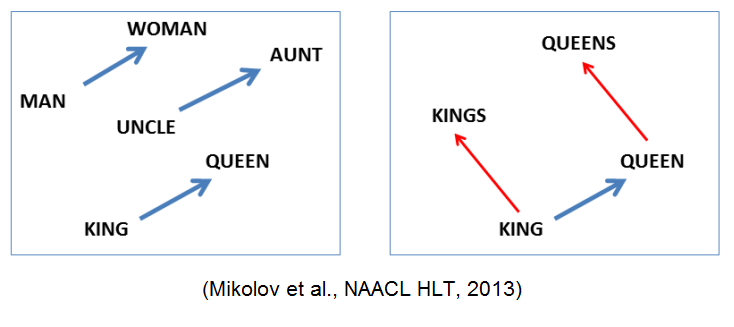
\includegraphics[width=10cm]{kingqueen.png}
	\caption{Semantic relationships between words as arrows in the vector space. \citep{WordVecLingReg}}
	\label{fig:w2vg}
\end{figure}

\begin{figure}[p]
	\centering
	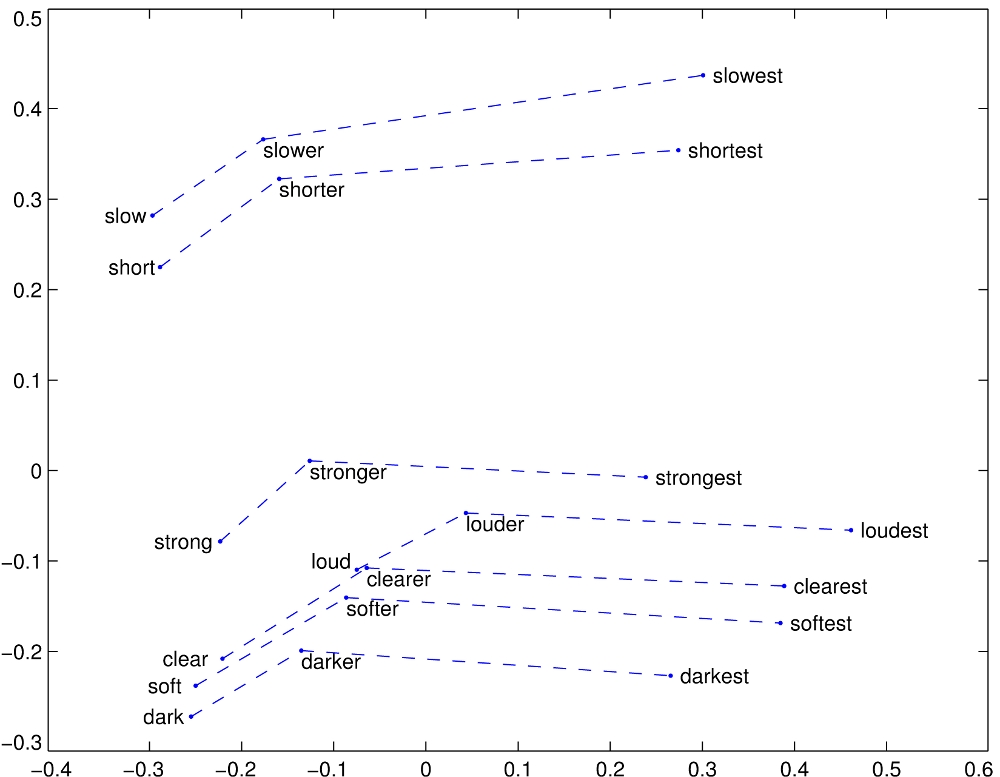
\includegraphics[width=10cm]{comparative_superlative.jpg}
	\caption{Semantic relationships between superlative adjectives as represented in the vector space.
		This is a 2D projection of the high-dimensional space that is designed to well preserve relative positions of the shown entities
		(so-called t-SNE 2D).
		\citep{Glove}}
	\label{fig:w2ver}
\end{figure}

\begin{figure}[p]
	\centering
	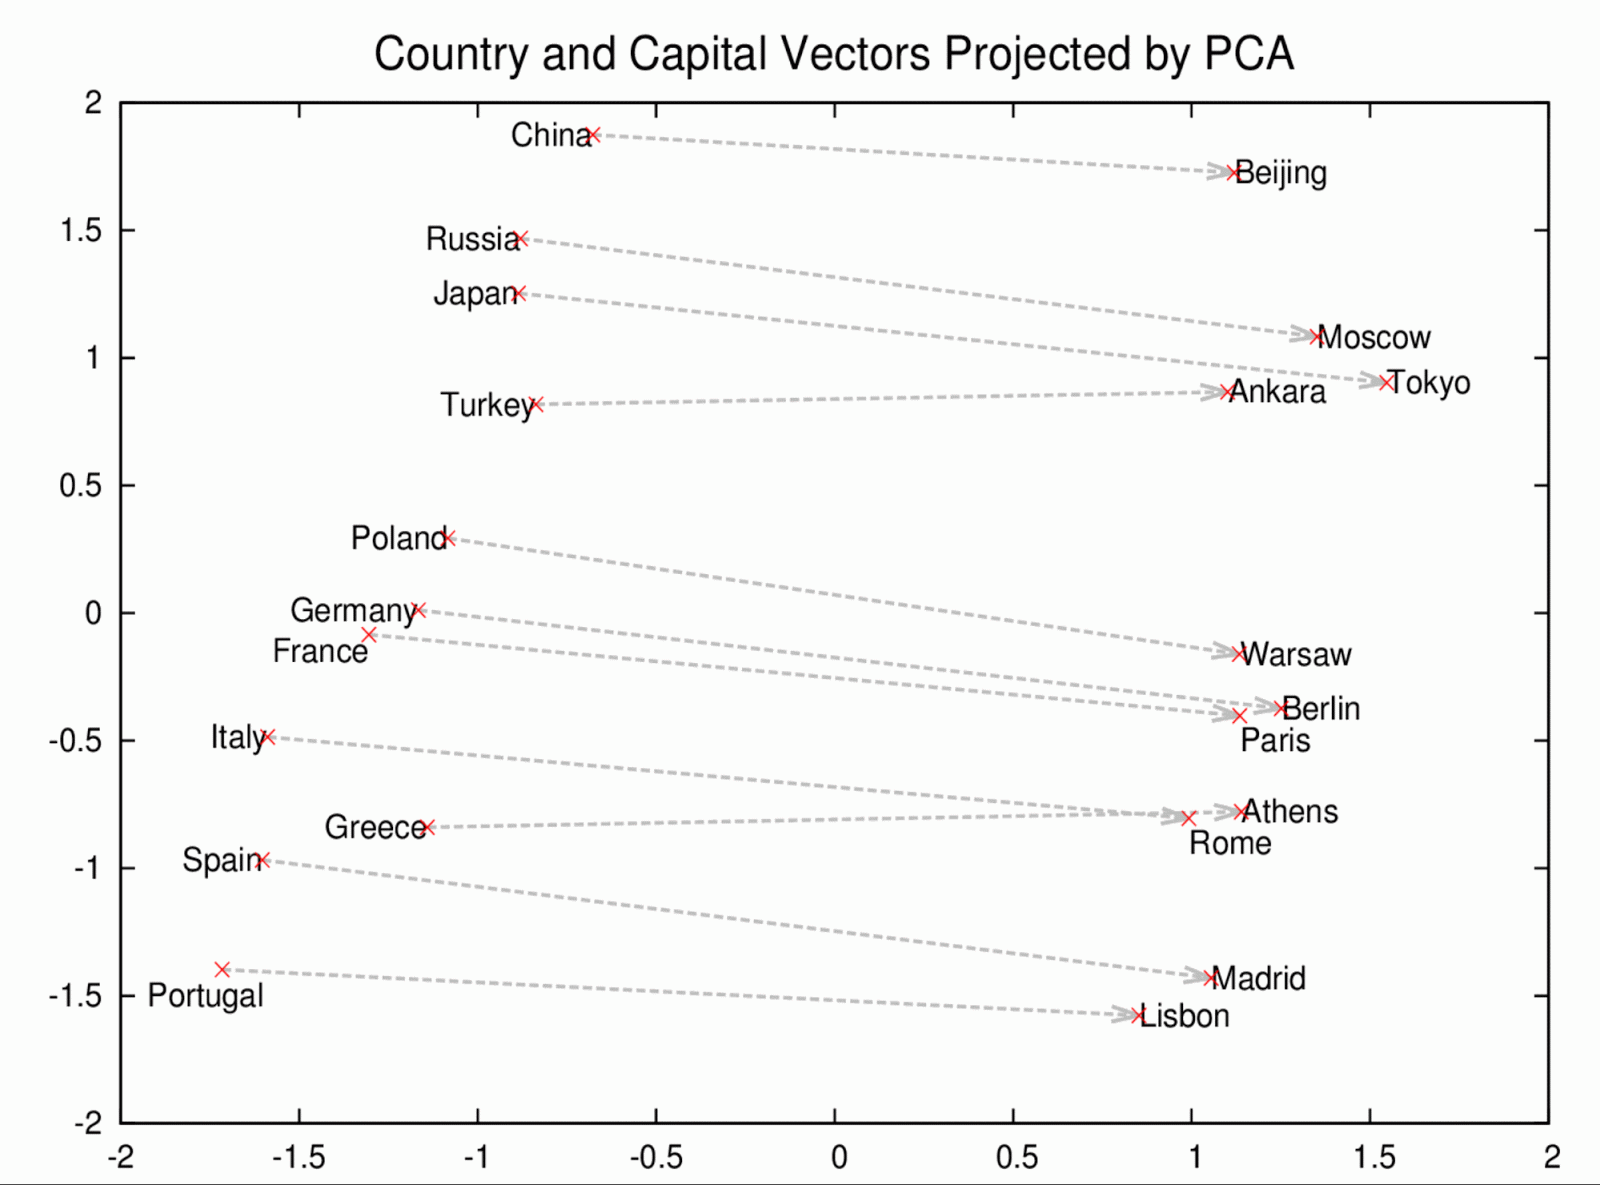
\includegraphics[width=11cm]{capitals.png}
	\caption{Mappings between countries and capitals, acquired entirely from the typical context of the respective words.
	This is again a 2D projection of the high-dimensional space, this time obtained by a PCA dimensionality reduction technique.
	\citep{DistReprComp}}
	\label{fig:w2vc}
\end{figure}

A lot of the current research focuses on the best ways to build up
vector representations of whole sentences and documents --- ranging
from simple averaging \citep{CNNSentClass,DefGen} (successful baselines)
to recurrent neural networks \citep{LISA,ShowAndTell}.
Many applications that rely on semantic understanding of word nuances
are popping up; this method became state-of-art for machine translation
\citep{LISA}, automatic image captioning \citep{ShowAndTell} and specific
types of question answering \citep{QANTA,DefGen,ReadAndComprehend}%
\footnote{The demo at \url{http://45.55.181.170/defgen/} is nice.}.
One open problem is efficient composition of vector embeddings for
common words with entities like numbers or proper names.
